\documentclass{include/thesisclass3}

\SelectLanguage{ngerman}
\usepackage{float}


% Titlepage settings
\newcommand{\praktikum}{Praktikum moderne Physik}
\newcommand{\autora}{Jens Schäfer}
\newcommand{\autorb}{Jan van der Linden}
\newcommand{\maila}{ugecd@student.kit.edu}
\newcommand{\mailb}{jan.vdlinden95@gmail.com}
\newcommand{\topic}{Spezifische Wärme}
\newcommand{\ptime}{10. Juli 2017}


% Shortcuts
\newcommand{\cc}{\cdot}
\newcommand{\rk}{\rangle}
\newcommand{\lk}{\langle}
\newcommand{\df}{\rightarrow}
\newcommand{\la}{\lambda}
\newcommand{\dd}{\text{d}}
\newcommand{\ehm}{\mathbbm{1}}
\newcommand{\p}{\partial}
\newcommand{\soll}{\overset{!}{=}}
\newcommand{\D}{\Delta}
\newcommand{\eps}{\epsilon}
\newcommand{\vektor}[3]{\begin{pmatrix} #1 \\ #2 \\ #3 \end{pmatrix}}
\newcommand{\vektorz}[2]{\begin{pmatrix} #1 \\ #2 \end{pmatrix}}
\newcommand{\Mat}[9]{\begin{pmatrix}#1&#2&#3\\#4&#5&#6\\#7&#8&#9\end{pmatrix}}
\newcommand{\Matz}[4]{\begin{pmatrix}#1&#2\\#3&#4\end{pmatrix}}
\newcommand{\e}[1]{\,\si{#1}}
\newcommand{\del}{\delta}
 


\begin{document}

	\FrontMatter
	% coordinates for background border
\newcommand{\diameter}{20}
\newcommand{\xone}{-15}
\newcommand{\xtwo}{160}
\newcommand{\yone}{15}
\newcommand{\ytwo}{-253}




\begin{titlepage}
    % background border
    \begin{tikzpicture}[overlay]
    \draw[color=gray]
            (\xone mm, \yone mm)
      -- (\xtwo mm, \yone mm)
    arc (90:0:\diameter pt)
      -- (\xtwo mm + \diameter pt , \ytwo mm)
        -- (\xone mm + \diameter pt , \ytwo mm)
    arc (270:180:\diameter pt)
        -- (\xone mm, \yone mm);
    \end{tikzpicture}



    % KIT image and sign for faculty of physics
    \begin{textblock}{10}[0,0](4.5,2.5)
        
\includegraphics[width=.25\textwidth]{include/kitlogo.pdf}
    \end{textblock}
    

    % horizontal line
    \begin{textblock}{10}[0,0](4.2,3.1)
        \begin{tikzpicture}[overlay]
        \draw[color=gray]
                (\xone mm + 5 mm, -12 mm)
          -- (\xtwo mm + \diameter pt - 5 mm, -12 mm);
        \end{tikzpicture}
    \end{textblock}



    % begin of text part
    \changefont{phv}{m}{n}    % helvetica
    \centering



    % thesis topic (en and ge)
    \vspace*{3cm}
    \Huge\praktikum\\



    % author name and institute
    \vspace*{5cm}
    
    \huge\topic\\






    % examiners (Referenten)
    \vspace*{3cm}
    \Large
    \begin{center}
        \begin{tabular}[ht]{l c l } 
  \autora & \hfill & \textit{\maila} \\
\autorb & \hfill & \textit{\mailb} \\
        
        \end{tabular}
    \end{center}



    % working time
    \vspace{2cm}
    \begin{center}
        \large{Durchgeführt am}: \ptime
    \end{center}



    % lowest text blocks concerning the KIT
    \begin{textblock}{10}[0,0](4,16.8)
        \tiny{KIT -- Universität des Landes Baden-Württemberg und nationales %
              Forschungszentrum in der Helmholtz-Gemeinschaft}
    \end{textblock}
    \begin{textblock}{10}[0,0](14,16.75)
        \large{\textbf{www.kit.edu}}
    \end{textblock}
\end{titlepage}

	\tableofcontents                  
	\newpage
	\MainMatter

%Protokollstart
\chapter{Theoretische Grundlagen der Thermodynamik}
Thermodynamische Systeme gehorchen den drei Hauptsätzen der Thermodynamik:
\begin{equation}
\dd U = \del Q + \del W = T\dd S - p \dd V
\end{equation} 
Zudem lassen sich diese Systeme vollständig durch Zustandsgleichungen, Variablen von Zustandsgleichungen werden Zustandsgrößen genannt und sind insbesondere. Ein Beispiel ist das ideale Gasgesetz:
\begin{equation}
pV=nRT
\end{equation}
\section{spezifische Wärme}
Die partielle Ableitung der Wärme nach der Temperatur bei einer festen Zustandsgröße wird spezifische Wärme genannt, sie sind Konstanten eines Stoffes. Es gilt:
\begin{align}
c_p &=\left(\frac{\del Q}{\del T}\right)_p\\
c_V &=\left(\frac{\del Q}{\del T}\right)_V = \left(\frac{\del U}{\del T}\right)_V\label{cv}
\end{align}
Die letztere Gleichheit folgt aus dem ersten Hauptsatz der Thermodynamik bei konstantem Volumen. \\
Mit dem Ausdehnungskoeffizienten $\alpha = \frac{1}{V} \cdot \left(\frac{\del V}{\del T}\right)$ und dem Kompressionsmodul \\$K=\frac{1}{\alpha}\cdot \left(\frac{\del p}{\del T}\right)_V$ lautet die Differenz der Wärmekapazitäten für Festkörper: 
\begin{equation}
c_p-c_V=T\alpha ^2 K
\end{equation}
Für Kupfer erhält man einen Numerischen Wert von 0.03 und nimmt für diesen Versuch die Gleichheit der spezifischen Wärmen für konstanten Druck und Volumen an.

\section{Debye-Modell}
Das Debye-Modell schlägt eine theoretische Herleitung für $c_V$ vor.

Dazu sei zunächst die Zustandsdichte $z(\omega)$ als Verteilungsfunktion der Eigenfrequenzen der Phononen im Kristall erklärt.
Um diese zu bestimmen hat Debye die folgenden Annahmen getroffen:
\begin{itemize}
\item jedes Atom hat drei Freiheitsgrade. In einem Kristall mit $N_A$ Atomen liegt die Anzal der Phononen deshalb bei $3N_A$\\
\item die bekannte lineare Dispersionsrelation für tiefe Frequenzen ist auch bei hohen Frequenzen gültig: $\omega = c k$\\
\item die maximal mögliche Eigenfrequenz des Schwingungsspektrums ist gegeben mit $\omega_D=\nu^3\sqrt{\frac{6 \pi ^2 N_A}{V}}$
\end{itemize}
Damit gilt für die Zustandsdichte
\begin{equation}
\int \limits_{0}^{\omega_D} \! z(\omega) \, \dd\omega = 3N_A
\end{equation}
Woraus sich die Zustandsdichte konkret berechnen lässt:
\begin{equation}
z(\omega)= \frac{9N_A}{\omega_D^3}\omega^2;\qquad 0\leq  \omega \leq \omega_D
\end{equation}

Es sei die innere Energie in einem Kristall gegeben mit
\begin{equation}
U= \int \limits_{\omega}^{}\! \frac{\hbar \omega}{e^{\frac{\hbar \omega}{k_B T}}-1} z(\omega)\dd \omega
\end{equation}
Die innere Energie kann nach Gleichung \ref{cv} zur Wärmekapazität mit konstantem Volumen umgeschrieben werden. Das dabei entstehende Integral wird numerisch gelöst, wobei Dulong-Petit  folgende Vereinfachungen und Lösungen geliefert hat, sei $\Theta_D=\frac{\hbar \omega_D}{k_B}$ so ergibt das Integral bei hohen Temperaturen:
\begin{equation}
c_v(T\ll\Theta_D)=c_{DP}=n\cdot 3N_Ak_b\approx 25\e{\frac{J}{mol\cdot K}}
\end{equation}
Mit n der Anzahl der Atome in der Basis eines Festkörpers.
Somit soll nach dem Gesetz von Dulong-Petit die Wärmekapazität bei hohen Temperaturen für Festkörper mit  Basis gleicher Ordnung gegen diese Konstante gehen. Für Temperaturen unterhalb $T=0.1\Theta_D$ ergibt das Integral hingegen
\begin{equation}
c_v=9N_Ak_B\frac{4\pi^4}{15}\left(\frac{T}{\Theta_D} \right)3
\end{equation}

\section{Phasenübergänge}


\chapter{Dysprosium und seine magnetischen Eigenschaften}
\chapter{Experiment}
Ziel des Experimentes ist es uns kräftig zu langweilen, obgleich relevante Themen für die kommende mündliche Prüfung vertieft werden.
\chapter{Auswertung}


\begin{figure}[ht]
	\begin{center}
		%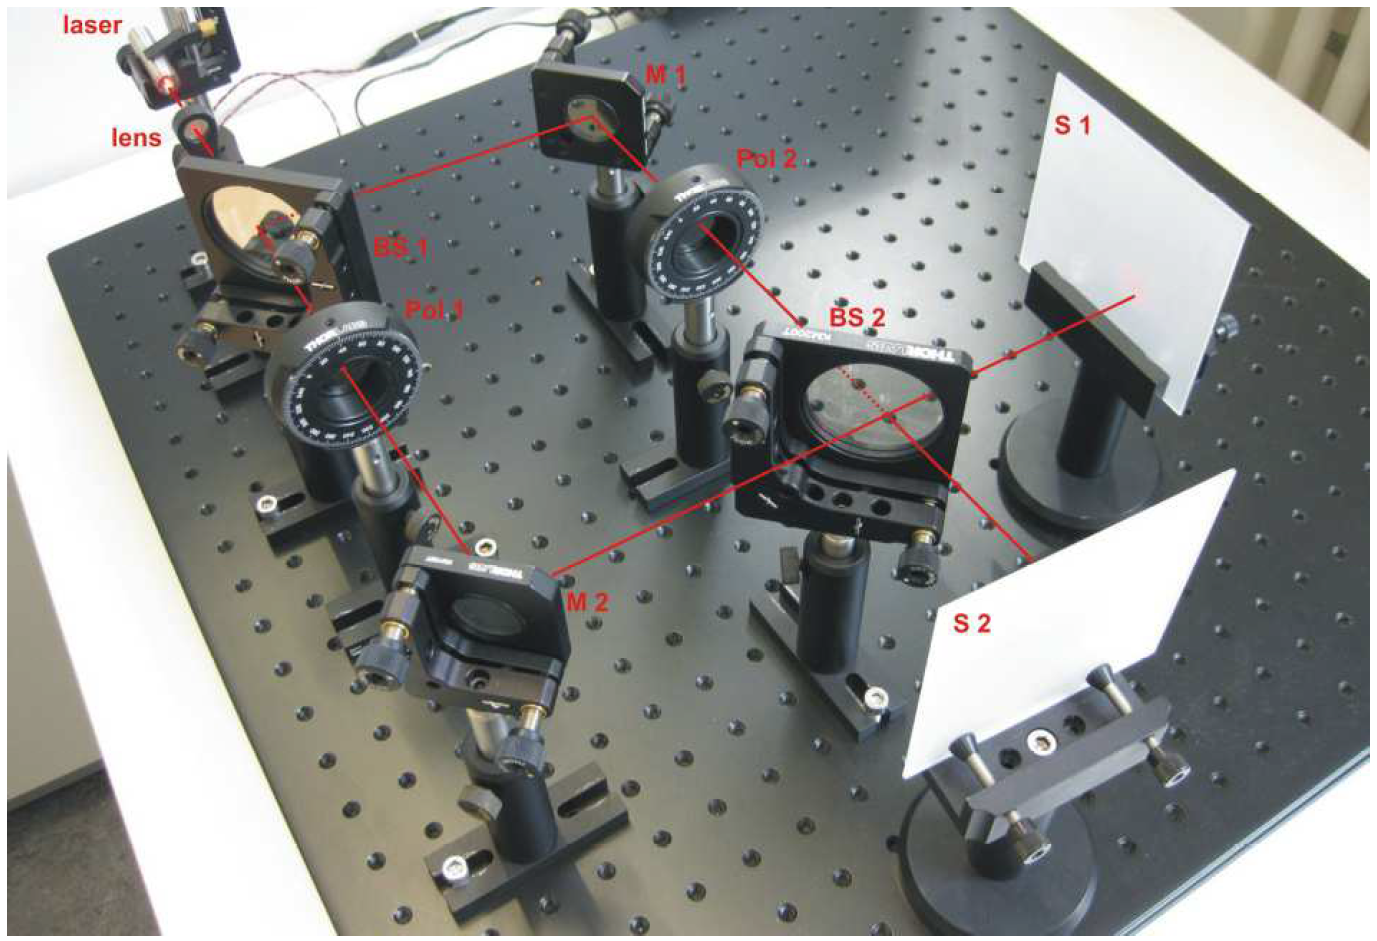
\includegraphics{images/Aufbau.png}
		\caption{Experimenteller Aufbau}
		\label{aufbau}
	\end{center}
\end{figure}

\end{document}
